OpenGL (Open Graphics Library) là một API đa nền tảng,
 đa ngôn ngữ cho render đồ họa vector 2D và 3D. API thường 
 được sử dụng để tương tác với bộ xử lý đồ họa (GPU), 
nhằm đạt được tốc độ render phần cứng

\begin {itemize}
\item API: Application Programming Interface: là một giao diện mà một hệ 
thống máy tính hay ứng dụng cung cấp để cho phép các yêu cầu dịch vụ 
có thể được tạo ra từ các chương trình máy tính khác, và/hoặc cho phép dữ liệu 
có thể được trao đổi qua lại giữa chúng. 
\item GPU: Graphics Processing Unit
Là bộ Vi xử lý chuyên phân tích những khối dữ liệu hình ảnh. 
GPU còn xử lý thông tin đa luồng, song song và bộ nhớ ở tốc độ cao.
 Kỹ thuật GPU đang dần trở nên dễ lập trình, cung cấp nhiều tiềm năng 
 cho việc tăng tốc xử lí cho nhiều chương trình với nhiều mục đích khác nhau,
  hơn cả chíp xử lí thông thường (CPUs).
  %chèn ảnh
\begin{figure}[ht]
\centering
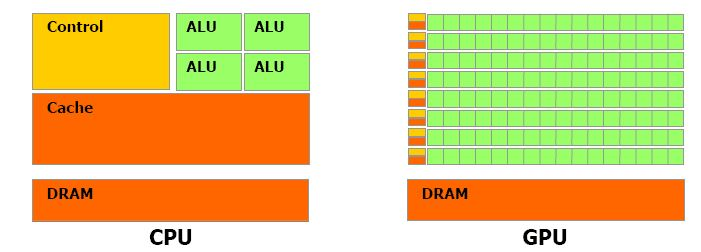
\includegraphics[scale=0.5]{1112_cpu-va-gpu-1.jpg}
\end{figure}


\item render:
gọi tắt là \textbf{kết xuất}, là một quá trình kiến tạo một hình ảnh từ
 một
 mô hình (hoặc một tập hợp các mô hình) thành một cảnh phim 
hoặc hình ảnh nào đó bằng cách sử dụng phần mềm máy tính. 

\begin{itemize}
    \item Mô hình: là mô tả của các đối tượng ba chiều bằng một ngôn ngữ 
    được định nghĩa chặt chẽ hoặc bằng một cấu trúc dữ liệu. Mô tả này bao 
    gồm các thông tin về hình học, điểm nhìn, chất liệu và bố trí ánh sáng 
    của đối tượng. Hình ảnh này có thể là một hình ảnh số (digital image) 
    hoặc một hình ảnh đồ họa điểm (raster graphics image). Thuật ngữ này
     có
     thể tương đồng 
    với "quá trình một họa sĩ vẽ" một phong cảnh nào đấy.

    \end{itemize}


\end{itemize}